\chapter{Evaluation}

In order to answer the questions raised in the introduction, the library \code{lox} is evaluated in this chapter.
This is done by, for example, comparing the execution speeds of \code{lox}, OpenMesh and PMP in several different benchmarks.
Furthermore, example code written with these three libraries is compared.  TODO: write this better.

Already during development, \code{lox}'s capabilities and ease of use were constantly tested by writing example programs and other tools.
As mentioned in the previous chapter, the command line utility \code{lox-cli} is developed alongside the main library to make sure the library offers all features such an application might require from it.
Additionally, an experimental application for rendering polygon meshes to SVG\footnote{Scalable Vector Graphic} files was developed outside of the main project, also assessing \code{lox}'s capabilities.
That application is not technically part of this master's thesis, but was used to create the images of meshes in this report, meaning they are all vector instead of pixel graphics.


\section{Execution Speed}

Geometry processing often has to deal with very large meshes, making the performance of geometry processing libraries very important.
Additionally, comparing the speed of \code{lox} to existing libraries is necessary in order to determine whether the abstractions employed by \code{lox} can be used without runtime overhead.
This chapter presents and discusses a number of different benchmarks.

All benchmarks were performed on a completely idle \textsf{Thinkpad T-460p} which, as already mentioned in chapter~4, contains an \textsf{Intel i7-6700\,HQ} and runs \textsf{Ubuntu 18.04}.
Of course, the notebook was \emph{not} running on battery during the benchmarks.
Additionally, at all times during the benchmarks, plenty of free main memory was available.
Each benchmark first executes the to be measured code 20~times as a warm-up without measuring anything.
Afterwards, the code is repeated 100 times and each iteration is measured individually.
From the 100 measured durations, the mean and standard deviation are calculated.

As already mentioned, the code, test meshes and raw results of all benchmarks can be found here: \url{https://github.com/LukasKalbertodt/masters-thesis}.

%TODO: Mention that DEM is not yet as optimized as it can be


\newpage
\subsection{Input/Output}

Some kind of IO can be found in most applications dealing with meshes, usually as the first and last step of said program.
While it is certainly not a particularly interesting processing step, its performance still is important to consider.
Different IO benchmarks were executed, covering this parameter space:

\begin{itemize}
  \item \textbf{Library/mesh implementation}: PMP, OpenMesh, \code{lox}'s half edge mesh (HEM), \code{lox}'s directed edge mesh (DEM) and \code{lox}'s shared vertex mesh (SVM) were tested.
  OpenMesh's and \code{lox}'s HEM were both configured for pure triangle meshes.
  \item \textbf{File format}: \textsc{Stl} and \textsc{Ply}.
  All benchmarks use little endian binary encoding.
  ASCII encoding only makes sense for tiny meshes in situations where it is necessary to manually inspect mesh data.
  Binary encoding is far more memory efficient and faster to read and write (independent of library).
  \item \textbf{Read or Write}
  \item \textbf{Mesh size}: the triangle meshes \enquote{cat} (59,292 faces) and \enquote{tiger} (232,956 faces) were tested.
  See \code{benchmarks/data/README.md} in the thesis' repository for more details.
\end{itemize}

Performing IO benchmarks comes with a few additional challenges.
Most importantly, it does not make sense to test the speed of the actual hardware disk as this is has little to do with the code performance.
To avoid this problem, a RAM disk\footnote{An allocated part of the main memory which is mounted into the file system.} can be used to store the input mesh files and as a target for all write operations.
However, this is not optimal as IO operations still have to communicate with the operating system, adding some overhead.

A better solution is to have an in-memory writer and reader in the benchmarking code to avoid interactions with the file system alltogether.
Benchmarks with both strategies were implemented for OpenMesh and \code{lox}, revealing that the RAM disk is roughly 1\% -- 6\% slower for read benchmarks and approximately 20\% -- 70\% slower for write benchmarks.
Unfortunately, PMP does not support reading from and writing to non-file streams.
To obtain a fair comparison between all three libraries, the in-memory disk solution was used for the main benchmark.

The results of the benchmark -- shown in figure~\ref{fig:io-benchmark} -- indicate a few different things:

\begin{itemize}
  \item \code{lox} outperforms the other libraries in all IO tasks, often significantly.
  \item In the \emph{read} benchmarks, \code{lox}'s HEM and DEM perform approximately equally well, with the SVM being notably faster.
  In the \emph{write} benchmarks however, the DEM performs as well as the SVM with the HEM being notably slower.
  This suggest that the DEM has the same speed as the HEM for mutating operations like \code{add_face}, but is faster for non-mutating operations.
  \item For IO operations, the choice of data structure has a notable effect on performance.
\end{itemize}

\begin{figure}[p]
  \centering
  \centerline{
    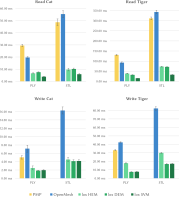
\includegraphics[width=1.1\textwidth]{svg2pdf/io-bench}
  }
  \vspace{1cm}
  \caption{
    Results of the IO benchmarks.
    The height of the bars is the mean of all measurements, the error bar displays the standard deviation.
    Values for \enquote{Write STL} benchmarks are missing for PMP, because the library only supports ASCII STL which is a lot slower than binary STL (those benchmarks took 500\,ms for \emph{cat} and 2000\,ms for \emph{tiger}).
  }
  \label{fig:io-benchmark}
\end{figure}

\newpage

\subsection{Algorithms}

\lipsum[1]


\newpage
\section{Example Code}

Speed is by far not the only factor determining the quality of a software library.
For example, if the library is hard to understand and use, the increase in development time usually outweighs the gains due to higher execution speed.
Unfortunately, it is often not possible to objectively evaluate a library's ease of use or the \enquote{readability} of its code -- particularly when comparing different languages.
However, to get a sense for the differences between \code{lox}, OpenMesh and PMP, this chapters shows a few example tasks realized with the different libraries.

Figure~\ref{fig:example-io} shows an example that reads the file \code{input.stl} and writes the mesh back into \code{output.ply}.
Two main differences between the \code{lox} version and the two other versions can be observed.
Firstly, with \code{lox}, the mesh is returned by the \code{read_file} function, while OpenMesh and PMP already require an instance of a mesh to read into, i.\,e. a variable has to created before reading.
Secondly, \code{lox}'s IO functions report errors via \code{io::Error} which includes information about the underlying cause, whereas OpenMesh's and PMP's functions signal success or failure via a single \code{bool} which does not carry any additional information.

In figure~\ref{fig:example-build}, code manually building a simple mesh is shown.
While most of the time, meshes are loaded from files, creating small meshes by hand is useful for examples and unit tests.
While the two snippets using OpenMesh and PMP are very similar, the code using \code{lox} differs substantially.
That is because with \code{lox}, mesh properties -- including vertex positions -- have to be stored in external property maps.
The \code{mesh!} macro is offered to make creating meshes more convenient by allowing the user to specify mesh connectivity and properties with a custom syntax.
However, it is possible that more methods are added to \enquote{fat meshes} in the future, which would allow them to be used just like the mesh types in OpenMesh and PMP.

The small code snippets in figure~\ref{fig:example-sqrt3} show how to run the $\sqrt{3}$-subdivision algorithm \cite{kobbelt20003} on a mesh.
In \code{lox}, the algorithm is a simple function, while the other libraries require the instantiation of a class, a method of which performs the actual algorithm.

Lastly, figure~\ref{fig:example-smooth} shows a simple smoothing algorithm (used for the \enquote{smooth} benchmarks in the previous section) that moves each vertex to the centroid of all neighbor vertices.
This shows a number of differences between the libraries.
For one, \code{lox}'s vertex iterator iterates over \code{VertexRef}s, allowing features like \code{v.adjacent_vertices()} and \code{v.is_boundary()}, while the other two libraries iterate over vertex handles.
In OpenMesh and PMP, the property map for the new positions is created from the mesh and filled afterwards; in \code{lox} it is created by collecting an iterator over \code{(VertexHandle, Point3)} pairs.
An iterator method \code{centroid} is offered by \code{lox}, while the versions implement that logic themselves.

In general, in situations in which \code{lox} code is more concise than equivalent code for the two other libraries, this advantage is mostly due to Rust's powerful iterator system.
It allows defining new methods (like \code{centroid}), but even the built-in methods can make some code notably shorter.
As another example, this code counts the number of boundary faces: \code{mesh.faces().filter(|f| f.is_boundary()).count()}.


\begin{figure}[p]
  \begin{minipage}{.04\textwidth}
    \rotatebox{90}{\textsf{\Large \textbf{lox}}}
  \end{minipage}
  \begin{minipage}{.9\textwidth}
    \begin{rustcode*}{fontsize=\footnotesize}
      use lox::{
          ds::SharedVertexMesh,
          fat::MiniMesh,
          io,
      };

      fn main() -> Result<(), io::Error> {
          type MyMesh = MiniMesh<SharedVertexMesh>;

          let mesh: MyMesh = io::read_file("input.stl")?;
          io::write_file(&mesh, "output.ply")?;

          Ok(())
      }
    \end{rustcode*}
  \end{minipage}\vspace{2mm}

  \begin{minipage}{.04\textwidth}
    \rotatebox{90}{\textsf{\Large \textbf{OpenMesh}}}
  \end{minipage}
  \begin{minipage}{.9\textwidth}
    \begin{cppcode*}{fontsize=\footnotesize}
      #include <iostream>
      #include <OpenMesh/Core/IO/MeshIO.hh>
      #include <OpenMesh/Core/Mesh/TriMesh_ArrayKernelT.hh>

      typedef OpenMesh::TriMesh_ArrayKernelT<> MyMesh;

      int main() {
          MyMesh mesh;
          if (!OpenMesh::IO::read_mesh(mesh, "input.stl")) {
              std::cerr << "Error reading file" << std::endl;
              return 1;
          }

          if (!OpenMesh::IO::write_mesh(mesh, "output.ply")) {
              std::cerr << "Error writing file" << std::endl;
              return 1;
          }
      }
    \end{cppcode*}
  \end{minipage}\vspace{2mm}

  \begin{minipage}{.04\textwidth}
    \rotatebox{90}{\textsf{\Large \textbf{PMP}}}
  \end{minipage}
  \begin{minipage}{.9\textwidth}
    \begin{cppcode*}{fontsize=\footnotesize}
      #include <iostream>
      #include <pmp/SurfaceMesh.h>

      using pmp::SurfaceMesh;

      int main() {
          SurfaceMesh mesh;
          if (!mesh.read("input.stl")) {
              std::cerr << "Error reading file" << std::endl;
              return 1;
          }

          if (!mesh.write("output.ply")) {
              std::cerr << "Error writing file" << std::endl;
              return 1;
          }
      }
    \end{cppcode*}
  \end{minipage}

  \caption{
    Example code loading one mesh file and writing the same mesh into another file.
    OpenMesh and PMP default to ASCII encoding when writing files, \codebox{lox} uses binary encoding by default.
    This is the only example that includes imports and function declarations.
  }
  \label{fig:example-io}
\end{figure}

\begin{figure}[p]
  \begin{minipage}{.04\textwidth}
    \rotatebox{90}{\textsf{\Large \textbf{lox}}}
  \end{minipage}
  \begin{minipage}{.9\textwidth}
    \begin{rustcode*}{fontsize=\footnotesize}
      let (mesh, vertex_positions) = mesh! {
          type: SharedVertexMesh,
          vertices: [
              v0: Point3::new(0.0, 0.0, 0.0),
              v1: Point3::new(0.0, 1.0, 0.0),
              v2: Point3::new(1.0, 0.0, 0.0),
              v3: Point3::new(1.0, 1.0, 0.0),
          ],
          faces: [
              [v0, v2, v1],
              [v2, v3, v1],
          ]
      };
      let mesh = MiniMesh { mesh, vertex_positions };
    \end{rustcode*}
  \end{minipage}\vspace{2mm}

  \begin{minipage}{.04\textwidth}
    \rotatebox{90}{\textsf{\Large \textbf{OpenMesh}}}
  \end{minipage}
  \begin{minipage}{.9\textwidth}
    \begin{cppcode*}{fontsize=\footnotesize}
      MyMesh mesh;

      const auto v0 = mesh.add_vertex(MyMesh::Point(0.0, 0.0, 0.0));
      const auto v1 = mesh.add_vertex(MyMesh::Point(0.0, 1.0, 0.0));
      const auto v2 = mesh.add_vertex(MyMesh::Point(1.0, 0.0, 0.0));
      const auto v3 = mesh.add_vertex(MyMesh::Point(1.0, 1.0, 0.0));

      mesh.add_face(v0, v2, v1);
      mesh.add_face(v2, v3, v1);
    \end{cppcode*}
  \end{minipage}\vspace{2mm}

  \begin{minipage}{.04\textwidth}
    \rotatebox{90}{\textsf{\Large \textbf{PMP}}}
  \end{minipage}
  \begin{minipage}{.9\textwidth}
    \begin{cppcode*}{fontsize=\footnotesize}
      SurfaceMesh mesh;

      const auto v0 = mesh.add_vertex(Point(0.0, 0.0, 0.0));
      const auto v1 = mesh.add_vertex(Point(0.0, 1.0, 0.0));
      const auto v2 = mesh.add_vertex(Point(1.0, 0.0, 0.0));
      const auto v3 = mesh.add_vertex(Point(1.0, 1.0, 0.0));

      mesh.add_triangle(v0, v2, v1);
      mesh.add_triangle(v2, v3, v1);
    \end{cppcode*}
  \end{minipage}

  \caption{
    Example code manually creating a mesh with two triangles.
  }
  \label{fig:example-build}
\end{figure}

\begin{figure}[p]
  \vspace{2mm}
  \rotatebox{0}{\textsf{\Large \textbf{lox}}}\\[-3mm]

  \hspace{.04\textwidth}
  \begin{minipage}{.9\textwidth}
    \begin{rustcode*}{fontsize=\footnotesize}
      algo::subdivision::sqrt3(&mut mesh.mesh, &mut mesh.vertex_positions, 1);
    \end{rustcode*}
  \end{minipage}\vspace{2mm}

  \vspace{2mm}
  \rotatebox{0}{\textsf{\Large \textbf{OpenMesh}}}\\[-3mm]

  \hspace{.04\textwidth}
  \begin{minipage}{.9\textwidth}
    \begin{cppcode*}{fontsize=\footnotesize}
      OpenMesh::Subdivider::Uniform::Sqrt3T<MyMesh, float>()(mesh, 1);
    \end{cppcode*}
  \end{minipage}\vspace{2mm}

  \vspace{2mm}
  \rotatebox{0}{\textsf{\Large \textbf{PMP}}}\\[-3mm]

  \hspace{.04\textwidth}
  \begin{minipage}{.9\textwidth}
    \begin{cppcode*}{fontsize=\footnotesize}
      auto sub = SurfaceSubdivision(mesh);
      sub.sqrt3();
    \end{cppcode*}
  \end{minipage}

  \caption{
    Example code executing the $\sqrt{3}$-subdivision algorithm offered by the libraries.
  }
  \label{fig:example-sqrt3}
\end{figure}

\begin{figure}[p]
  \begin{minipage}{.04\textwidth}
    \rotatebox{90}{\textsf{\Large \textbf{lox}}}
  \end{minipage}
  \begin{minipage}{.9\textwidth}
    \begin{rustcode*}{fontsize=\footnotesize}
      mesh.vertex_positions = mesh.mesh.vertices().map(|v| {
          let old_pos = mesh.vertex_positions[v.handle()];
          let new_pos = if v.is_boundary() {
              old_pos
          } else {
              v.adjacent_vertices()
                  .map(|n| mesh.vertex_positions[n.handle()])
                  .centroid()
                  .unwrap()
          };
          (v.handle(), new_pos)
      }).collect();
    \end{rustcode*}
  \end{minipage}\vspace{2mm}

  \begin{minipage}{.04\textwidth}
    \rotatebox{90}{\textsf{\Large \textbf{OpenMesh}}}
  \end{minipage}
  \begin{minipage}{.9\textwidth}
    \begin{cppcode*}{fontsize=\footnotesize}
      auto cogs = OpenMesh::makeTemporaryProperty<VertexHandle, MyMesh::Point>(mesh);
      for (const auto& vh : mesh.vertices()) {
          if (mesh.is_boundary(vh)) {
              cogs[vh] = mesh.point(vh);
          } else {
              cogs[vh] = {0, 0, 0};
              int valence = 0;
              for (const auto& vvh : mesh.vv_range(vh)) {
                  cogs[vh] += mesh.point(vvh);
                  valence += 1;
              }
              cogs[vh] /= valence;
          }
      }

      for (const auto& vh : mesh.vertices()) {
          mesh.point(vh) = cogs[vh];
      }
    \end{cppcode*}
  \end{minipage}\vspace{2mm}

  \begin{minipage}{.04\textwidth}
    \rotatebox{90}{\textsf{\Large \textbf{PMP}}}
  \end{minipage}
  \begin{minipage}{.9\textwidth}
    \begin{cppcode*}{fontsize=\footnotesize}
      auto new_pos = mesh.add_vertex_property<Point>("v:new_pos");
      auto points = mesh.get_vertex_property<Point>("v:point");

      for (const auto v: mesh.vertices()) {
          if (mesh.is_boundary(v)) {
              new_pos[v] = points[v];
          } else {
              auto total_displacement = vec3(0, 0, 0);
              size_t valence = 0;
              for (const auto neighbor: mesh.vertices(v)) {
                  total_displacement += points[neighbor];
                  valence += 1;
              }
              new_pos[v] = total_displacement / valence;
          }
      }

      for (const auto v: mesh.vertices()) {
          points[v] = new_pos[v];
      }
      mesh.remove_vertex_property(new_pos);
    \end{cppcode*}
  \end{minipage}

  \caption{
    Example code performing a simple mesh smoothing.
  }
  \label{fig:example-smooth}
\end{figure}


\newpage
\section{Summary}

% As can be seen from this chapter, \code{lox} is certainly usable and offers the basic features expected from a mesh processing library.
As can be seen from the previous chapters, \code{lox} is a viable mesh processing library which offers the basic features expected from such a package.
It allows implementing sophisticated mesh algorithms (like $\sqrt{3}$-subdivision) and it has been successfully used to create two useful applications: \code{lox-cli} and an SVG renderer.
Compared to two existing \cpp libraries, OpenMesh and PMP, \code{lox} has advantages in some areas but disadvantages in others.
Currently, \code{lox} is not as complete as the other two libraries, particularly regarding mesh algorithms.
Naturally, the library is also not nearly as mature as OpenMesh.

The main benefit of \code{lox} comes from having achieved its central goal:
to provide an abstraction over different data structures and let the programmer decide which data structure to use in which situation.
This works well and does not incur any significant runtime overhead, as shown in the benchmarks where \code{lox} outperforms the other libraries.
Additional advantages of \code{lox} include the superior performance of IO operations and being able to use Rust, which in itself has several advantages over \cpp.

In some areas, \code{lox} could not improve the status-quo yet.
For example, while some operations can be expressed more concisely due to \code{lox}'s use of Rust features, some other tasks require slightly more code using \code{lox} than existing \cpp libraries.
Particularly problematic for \code{lox} is the use of indices to refer to data, because generally, each array access has to be bound checked to avoid reading uninitialized memory.
Unfortunately the optimizer is not able to remove those bound checks most of the time in the context of this library, meaning that this safety guarantee incurs notable runtime overhead.
This can be seen in some of the benchmarks.
The problem could potentially be solved by using Rust's type system to \enquote{sign} (or \enquote{brand}) valid indices at compile time, a pattern explored in \cite[Chapter~6.3]{beingessner2016you}.
This, however, was not attempted in this thesis.
